
\title{Taler: \\ Usable, privacy-preserving payments for the Web}
 \author{
 Jeffrey Burdges \\ \and
 Florian Dold \\ \and
 Christian Grothoff \\ \and
 Marcello Stanisci
}
\date{\today}

\documentclass[twoside,letterpaper]{sigalternate}
\usepackage[margin=1in]{geometry}
\usepackage[utf8]{inputenc}
\usepackage{url}
\usepackage{tikz}
\usepackage{listings}
\usepackage{graphicx}
\usepackage{wrapfig}
\usepackage{caption}
\usepackage{subcaption}
\usepackage{url}
%\usepackage{dblfloatfix}

\usetikzlibrary{shapes,arrows}
\usetikzlibrary{positioning}
\usetikzlibrary{calc}

\begin{document}
\maketitle

\section{System overview}

Content and services provided on the internet, such as reading a blog post or
sending an email, tend to be of very small monetary value compared to
traditional financial transactions.  Currently the majority of online offerings
are financed via advertisements.  Any alternatives must reduce the mental
and technical overheads of existing payment systems to handle micro-payments.
Addressing this problem is urgent because advertising revenue is declining,
% \cite{??peakads??},
% It's possibly being erroded by ad-blocking technology
% but arguably ad-blocking is a way to save it. \cite{??AskJeff??}
and the Big Data business model where citizens pay with their
private information in combination with the deep state hastens our society's
regression towards post-democracy~\cite{rms2013democracy}.

Taler is a new electronic online payment system that provides
anonymity for customers.  Here, {\em anonymous} simply means that the
payment system does not involve any personal information from the
customer, and that different transactions by the same customer are
unlinkable.  For strong anonymity, Taler usually needs to be used in
combination with existing techniques, such as Tor and \cite{apod}, to
avoid circumstances leaking information about the customer's identity.  
The facts that the user does not need to authenticate, and that the merchant
thus never learns sensitive personal information about the customer,
improves usability and security: the payment process is simplified, the
merchant's security requirements are dramatically reduced and the customer's
risk of identity theft does not accumulate with every (micro-)payment.
% The preceeding is a run-on but I didn't fix it

Taler uses blind signatures~\cite{chaum1983blind} to create digital
coins, and a novel ``refresh'' protocol to allow giving change and
refunds while maintaining unlinkability.  We will not go into the
details of Taler's cryptographic protocols here\footnote{Full
documentation at \url{https://api.taler.net/}} and instead focus on the
high-level concepts to explain how the system works from the
perspective of customers and merchants in the Taler
system (Figure~\ref{fig:system}).
% "... and how it contributes to customer privacy"?

\begin{figure}[t!]
\centering
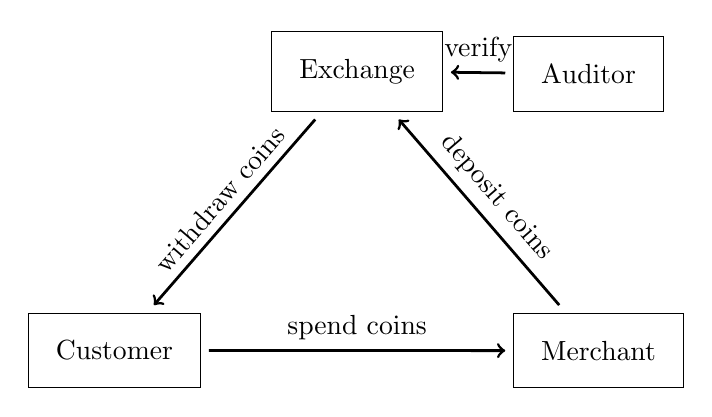
\begin{tikzpicture}
 \tikzstyle{def} = [node distance=3em and 5em, inner sep=1em, outer sep=.3em];
 \node (origin) at (0,0) {};
 \node (exchange) [def,above=of origin,draw]{Exchange};
 \node (customer) [def, draw, below left=of origin] {Customer};
 \node (merchant) [def, draw, below right=of origin] {Merchant};
 \node (auditor) [def, draw, above right=of origin]{Auditor};

 \tikzstyle{C} = [color=black, line width=1pt]

 \draw [<-, C] (customer) -- (exchange) node [midway, above, sloped] (TextNode) {withdraw coins};
 \draw [<-, C] (exchange) -- (merchant) node [midway, above, sloped] (TextNode) {deposit coins};
 \draw [<-, C] (merchant) -- (customer) node [midway, above, sloped] (TextNode) {spend coins};
 \draw [<-, C] (exchange) -- (auditor) node [midway, above, sloped] (TextNode) {verify};

\end{tikzpicture}
\caption{Taler system overview.}
\label{fig:system}
\end{figure}

\section{Customer perspective}

In Taler, customers use a {\em wallet} to withdraw, hold, and spend coins.
Withdrawing coins requires the customer to authenticate and to optionally
authorize the specific transaction, e.g. via a PIN/TAN method as commonly used
by banks.  Afterwards, the customer can anonymously spend their coins by visiting
merchants without having to authenticate for each transaction.

The wallet is implemented as a cross-platform browser extension.  All
cryptographic operations and access to sensitive data are executed in a
component that is isolated from websites the user visits.

By necessity, the wallet leaks one bit of information to websites that the user
visits, namely whether the wallet is installed and activated by the user.
Websites cannot access the customer's balance or purchase history.  This
however also means that all cryptographic tokens of value are kept locally, and
the customer is responsible for not losing them.  Future versions of the wallet
will provide encrypted backups and synchronization between the wallets of a
user.

A common activity for online content is sharing and bookmarking.
Taler specifically provides support to make this easy for the user.
A resource that was purchased is identified by a unique \emph{fulfillment URL}
for each purchase of the resource.


\begin{figure*}[h!]
\begin{center}
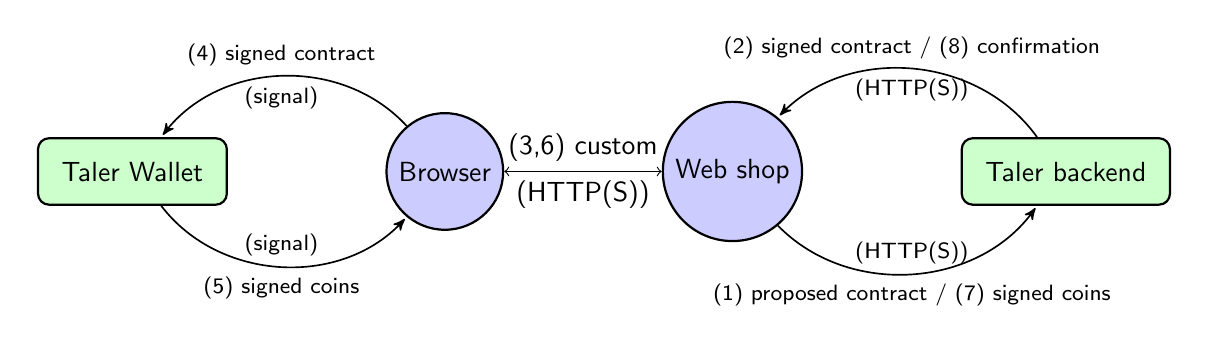
\begin{tikzpicture}[
  font=\sffamily,
  every matrix/.style={ampersand replacement=\&,column sep=2cm,row sep=2cm},
  source/.style={draw,thick,rounded corners,fill=green!20,inner sep=.3cm},
  process/.style={draw,thick,circle,fill=blue!20},
  sink/.style={source,fill=green!20},
  datastore/.style={draw,very thick,shape=datastore,inner sep=.3cm},
  dots/.style={gray,scale=2},
  to/.style={->,>=stealth',shorten >=1pt,semithick,font=\sffamily\footnotesize},
  every node/.style={align=center}]

  % Position the nodes using a matrix layout
  \matrix{
    \node[source] (wallet) {Taler Wallet};
      \& \node[process] (browser) {Browser};
      \& \node[process] (shop) {Web shop};
      \& \node[sink] (backend) {Taler backend}; \\
  };

  % Draw the arrows between the nodes and label them.
  \draw[to] (browser) to[bend right=50] node[midway,above] {(4) signed contract}
      node[midway,below] {(signal)} (wallet);
  \draw[to] (wallet) to[bend right=50] node[midway,above] {(signal)}
      node[midway,below] {(5) signed coins} (browser);
  \draw[<->] (browser) -- node[midway,above] {(3,6) custom}
      node[midway,below] {(HTTP(S))} (shop);
  \draw[to] (shop) to[bend right=50] node[midway,above] {(HTTP(S))}
      node[midway,below] {(1) proposed contract / (7) signed coins} (backend);
  \draw[to] (backend) to[bend right=50] node[midway,above] {(2) signed contract / (8) confirmation}
      node[midway,below] {(HTTP(S))} (shop);
\end{tikzpicture}
\end{center}
 \caption{Both the customer's client and the merchant's server execute
          sensitive cryptographic operations in a secured
          background/backend that is protected against direct access.
     % THIS SENTENCE DOES NOT MAKE SENSE : 
          Interactions between the Taler components
          (Figure~\ref{fig:system}) are not shown.  Existing system
          security mechanisms are used to isolate the cryptographic
          components (boxes) from the complex rendering logic
          of existing Web applications (circles).}
 \label{fig:frobearch}
\end{figure*}

% maybe mention division into two phases (a) contract offer/accept
% and (b) contract execution/replay

% How far does this allow the merchant 
Should the session state that allows the user to access the content be lost,
visiting the fulfillment URL will transparently restore the session state by
transparently replaying the payment with the same digital value tokens from the
user's wallet.  Replaying a contract is only allowed from the domain that the
contract originated from, and thus does not allow arbitrary websites to obtain
information about previous purchases that the customer made.  Sharing the
fulfillment URL with a user that did not pay for the associated digital
contract will result in the expected behavior, namely that they receiving a new
instance of the digital contract with the opportunity to pay for it.

% idea while writing this:  why do we need a correlation id
% if we already have the url? i.e. the non-fulfillment URL
% that just identifies the resource ...

The case where a user already payed for a resource and then visits
the resource URL (instead of the fulfillment URL) after losing temporary
session state is also handled as expected, since the wallet component will
look for contracts that refer to the same resource.

While Taler is designed to work well with digital resources on the web,
it can also be used for more traditional purchases.  The resource that
is being payed for then represents the shopping cart of items that
are being purchased.

%\newpage
\section{Merchant perspective}



%\begin{figure}[b!]
%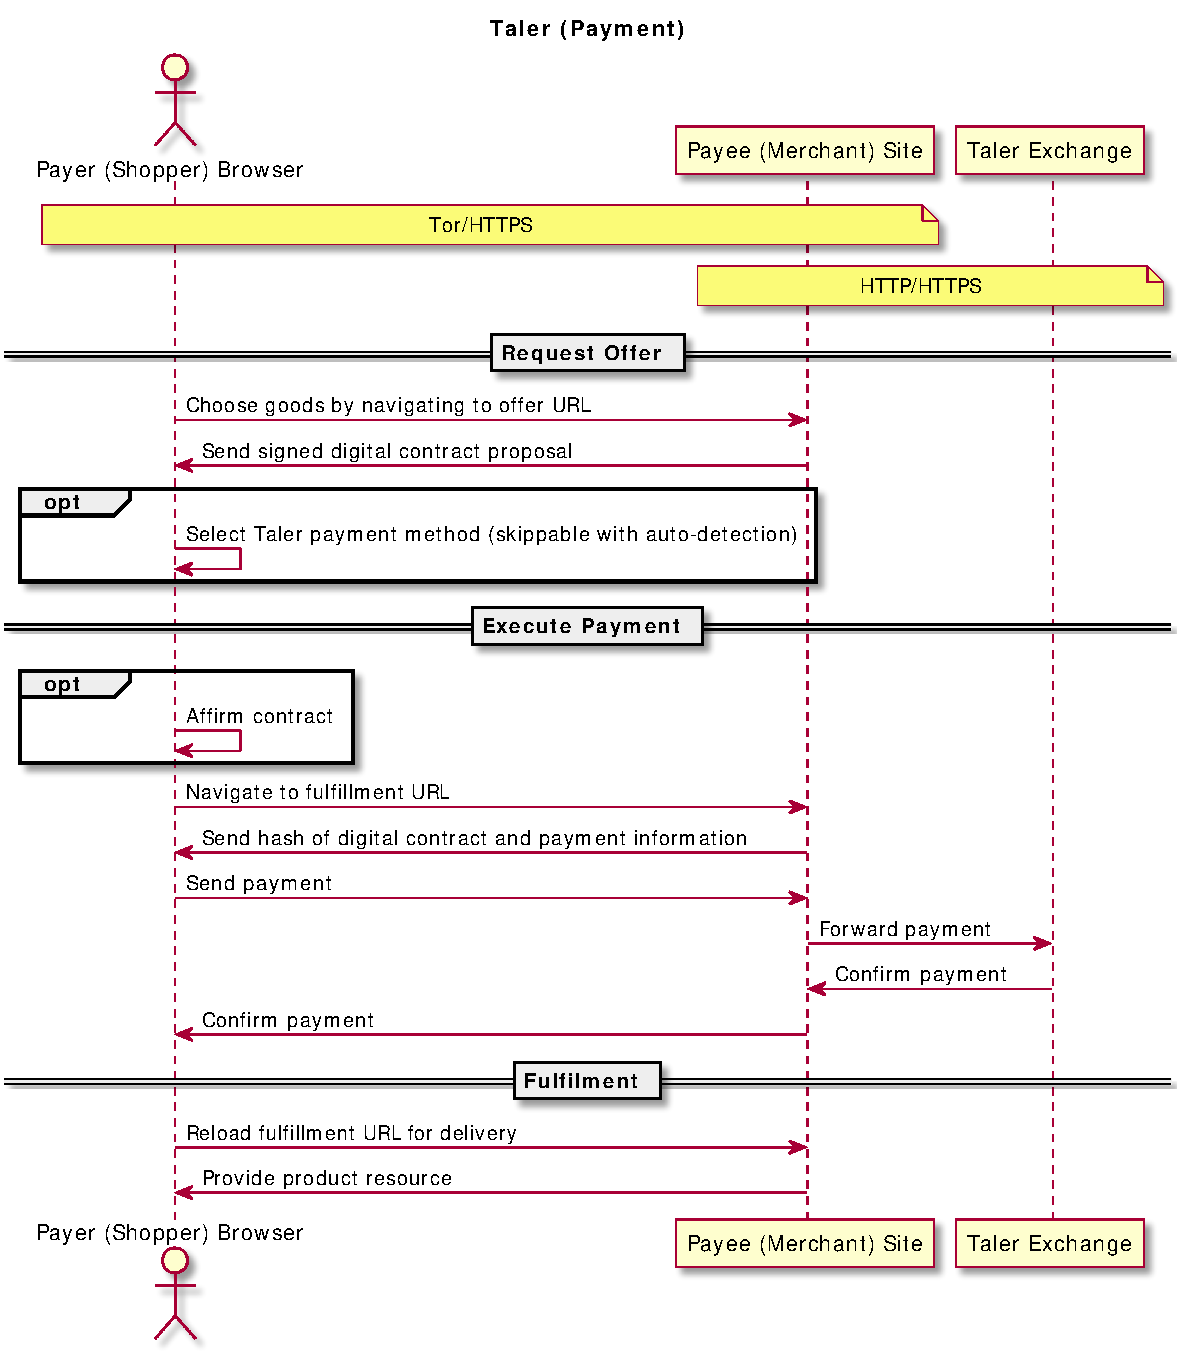
\includegraphics[width=0.45\textwidth]{figs/taler-pay.pdf}
%\caption{Payment processing with Taler.}
%\label{fig:taler-pay}
%\end{figure}


A new payment system must also be easy to integrate and deploy for merchants.
Figure~\ref{fig:frobearch} shows how the security critical payment components of
Taler interact with the logic of existing Web shops.  First, the Web shop
front-end is responsible for constructing the shopping cart.  For this,
the shop front-end generates the usual Web pages which are shown to the
user's browser client front-end.  Once the order has been constructed,
the shop front-end gives a {\em proposed contract} in JSON format to
the payment backend, which signs it and returns it to the front-end.
The front-end then transfers the signed contract over the network, and
passes it to the wallet.  Here, the wallet operates from a secure
background context on the client side, which allows the user to securely
accept the payment, and to perform the cryptographic operations in a
context that is protected from the Web shop.  If the user accepts, the
resulting signed coins are transferred from the client to the server,
again by a protocol that the merchant can customize to fit the
existing infrastructure.



Instead of adding any cryptographic logic to the merchant front-end,
the generic Taler merchant backend allows the implementor to delegate
handling of the coins to the payment backend, which validates the
coins, deposits them at the exchange, and finally validates and
persists the receipt from the exchange.  The merchant backend then
communicates the result of the transaction to the front\-end, which is
then responsible for executing the business logic to fulfill the
order.
As a result of this setup, the cryptographic details of the
Taler protocol do not have to be re-implemented by each merchant.
Instead, existing Web shops implemented in a multitude of programming
languages can rather trivially add support for Taler by {\bf (1)} upon
request, generating a contract in JSON based on the shopping cart,
{\bf (2)} allowing the backend to sign the contract before sending it
to the client, {\bf (7)} passing coins received in payment for a
contract to the backend and {\bf (8)} executing fulfillment business
logic if the backend confirms the validity of the payment.


To setup a Taler backend, the merchant only needs to configure it with the
respective wire transfer routing details, such as an IBAN number.  The
customer's authentication of the Web shop continues to rely upon
\mbox{HTTPS}/X.509.

\section{Conclusion}

We encourage everyone to try our prototype for Taler
at \url{https://demo.taler.net/}.

% FIX ME : Can we say that a HotPETS discussion would be useful somehow?
% Like explain that we want input on deployment scenarios. 


% These APIs are all RESTful in the modern sense because that greatly
% simplify integrating Taler with web shops and browsers.

\section*{Acknowledgements}

This work benefits from the financial support of the Brittany Region
(ARED 9178) and a grant from the Renewable Freedom Foundation.


\bibliographystyle{abbrv}
\bibliography{ui,btc,taler,rfc}

\end{document}
